\chapter{Materiales y métodos} 

% ------------------------------------------------------------------------------------------------------------
% ------------------------------------------------------------------------------------------------------------

\section{Conjunto de datos disponibles}

Disponemos de un conjunto de datos compuesto por radiografías panorámicas maxilofaciales de individuos de 12 países distintos (véase en la tabla \ref{tab:instituciones_fuente_dataset}), obtenidas con distintos modelos de máquinas de rayos X%
\footnote{
    Los modelos empleados fueron: \textit{Planmeca Promax Digital Panoramic}; \textit{Sirona ORTHOPHOS-XG}, \textit{ORTHOPHOS-DS}, y \textit{SIDEXIS}. Las constantes radiológicas usadas fueron de 66 a a 70 kV, 7 a 11 mA, y 15 s.
}.
Este conjunto de datos ha sido sido proporcionado por Panacea Cooperative Research, empresa \textit{spin-off} de la Universidad de Granada.  

\begin{table}[h]
    \begin{tabular}{@{}clc@{}}
    \toprule
    País                                                            & Instituciones                                                                                                                                                            & Nº de ejemplos \\ \midrule
    \begin{tabular}[c]{@{}c@{}}Bosnia y \\ Herzegovina\end{tabular} & Universidad de Sarajevo                                                                                                                                                  & 882            \\ \hline
    Botsuana                                                        & \begin{tabular}[c]{@{}l@{}}Dos clínicas dentales privadas en \\ Garobone\end{tabular}                                                                                    & 1242           \\ \hline
    Chile                                                           & \begin{tabular}[c]{@{}l@{}}Dos clínicas dentales privadas en \\ Santiago y Rancagua\end{tabular}                                                                         & 1016           \\ \hline
    \begin{tabular}[c]{@{}c@{}}República \\ Dominicana\end{tabular} & \begin{tabular}[c]{@{}l@{}}Tres clínicas dentales privadas en \\ Santo Domingo, La Vega y Santiago\end{tabular}                                                          & 541            \\ \hline
    Japón                                                           & \begin{tabular}[c]{@{}l@{}}Department of Forensic Sciences, \\ Iwate Medical University, Iwate\end{tabular}                                                              & 1045           \\ \hline
    Corea del Sur                                                   & Catholic University of Korea, Seoul                                                                                                                                      & 500            \\ \hline
    Malasia                                                         & \begin{tabular}[c]{@{}l@{}}Faculty of Dentistry Universiti Teknologi \\ MARA Selangor Branch, Selangor\end{tabular}                                                      & 667            \\ \hline
    Turquía                                                         & \begin{tabular}[c]{@{}l@{}}Department of Dentomaxillofacial \\ Radiology, Baskent University, Turkey\end{tabular}                                                        & 2323           \\ \hline
    Uganda                                                          & \begin{tabular}[c]{@{}l@{}}Department of Dental Morphology with \\ the Université Claude Bernard Lyon 1, \\Faculté d’odontologie, Lyon\end{tabular}                      & 283            \\ \hline
    Italia                                                          & \begin{tabular}[c]{@{}l@{}}Department of Surgical Sciences, \\ University of Cagliari\end{tabular}                                                                       & 173            \\ \hline
    Kosovo                                                          & \begin{tabular}[c]{@{}l@{}}University Dentistry Clinical Center, \\ Pristina\end{tabular}                                                                                & 1397           \\ \hline
    Líbano                                                          & Clínica dental privada en Beirut                                                                                                                                         & 690            \\ \bottomrule
    \end{tabular}
    \caption[
        Lista de instituciones participantes en la recolección de los datos e imágenes dentales utilizados en el trabajo.
    ]{   
        Lista de instituciones participantes en la recolección de los datos e imágenes dentales utilizados en el trabajo.
    }
    \label{tab:instituciones_fuente_dataset}
\end{table}

Este \textit{dataset} incluye:

\begin{itemize}

    \item datos tabulares (en formato CSV), donde cada fila representa un ejemplo (un individuo), con los siguientes campos: un identificador único, sexo del individuo, edad del individuo y ``sample'' (clasificación según el origen geográfico de la radiografía).

    \item imágenes bidimensionales de radiografías panorámicas maxilofaciales, con una imagen asociada a cada individuo mediante su ID único. 

\end{itemize}

Se proporcionan los datos ya preprocesados, por lo que no es necesario realizar tareas adicionales de limpieza o transformación previa antes de su análisis.

Se ha ignorado el campo ``sample'', dado que se trata de una asignación sesgada y no representa necesariamente una clasificación fiable del origen poblacional de los individuos. Por tanto, este campo no se emplea en el análisis ni en el entrenamiento de los modelos, centrándose exclusivamente en las variables de edad, sexo e imagen.

En el \textit{dataset} hay un total de 10 739 ejemplos, de los que 5756 son de individuos de sexo femenino y 4983 de sexo masculino. Las edades mínima y máxima son 14 y 26 años, respectivamente, y la media son 19.13 años. En la Figura \ref{fig:histogram_ages} se observa que el número de ejemplos por edad se mantiene relativamente constante desde los 14 hasta los 21 años, a partir de los cuales disminuye progresivamente, con una representación notablemente menor en los grupos de 24, 25 y 26 años.
 
\begin{figure}[h]
    \centering
    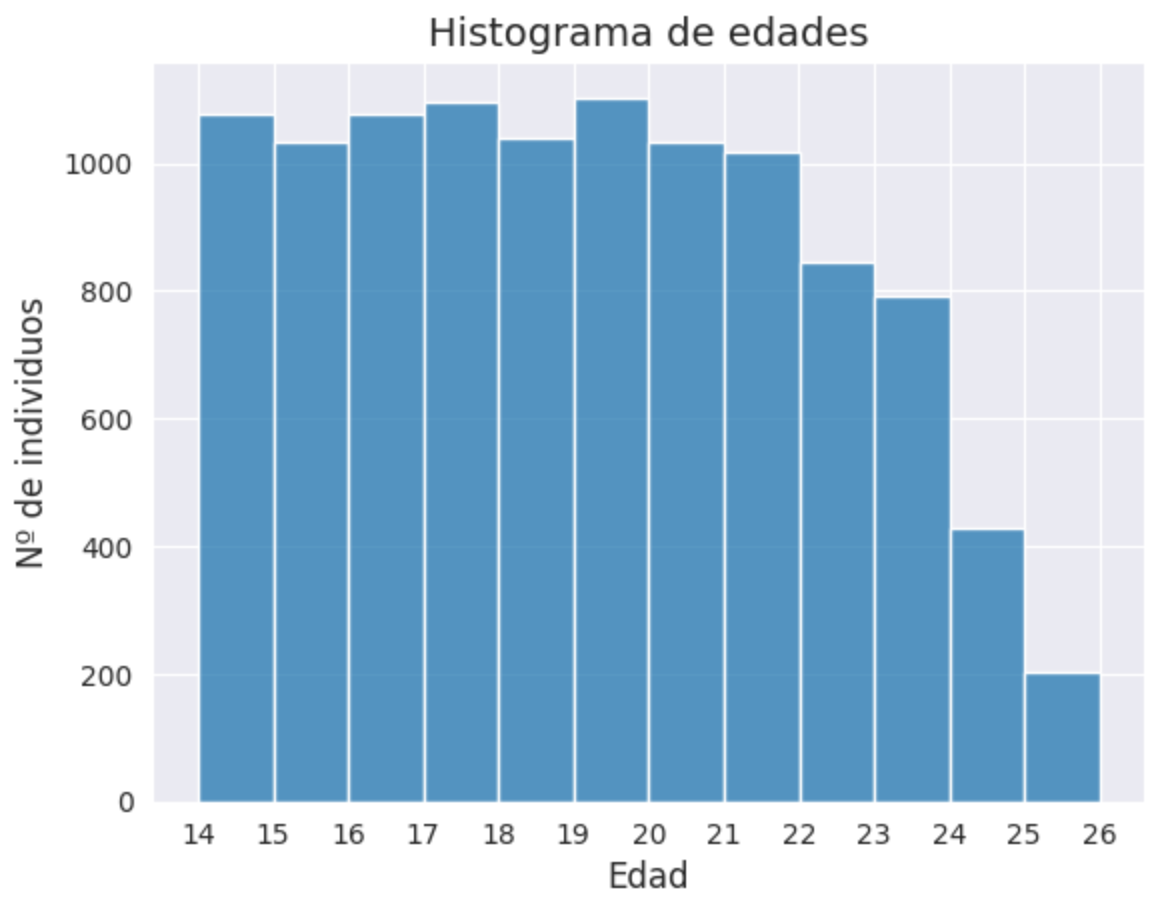
\includegraphics[width=0.7\textwidth]{capitulos/cap_04/imagenes/histogram_ages.png}
    \caption[
        Histograma de edad de los individuos del conjunto de datos disponible.
    ]{
        Histograma de edad de los individuos del conjunto de datos disponible. 
    } 
    \label{fig:histogram_ages}
\end{figure}

En la Figura \ref{fig:kde_and_boxplot_ages_sex} podemos comprobar cómo en términos relativos la distribución de edad por sexo es muy similar, compartiendo ambas prácticamente el mismo rango de edades y patrones de dispersión, sin observarse diferencias sustanciales en la mediana ni en la forma general de las distribuciones.

\begin{figure}[H]
    \centering
    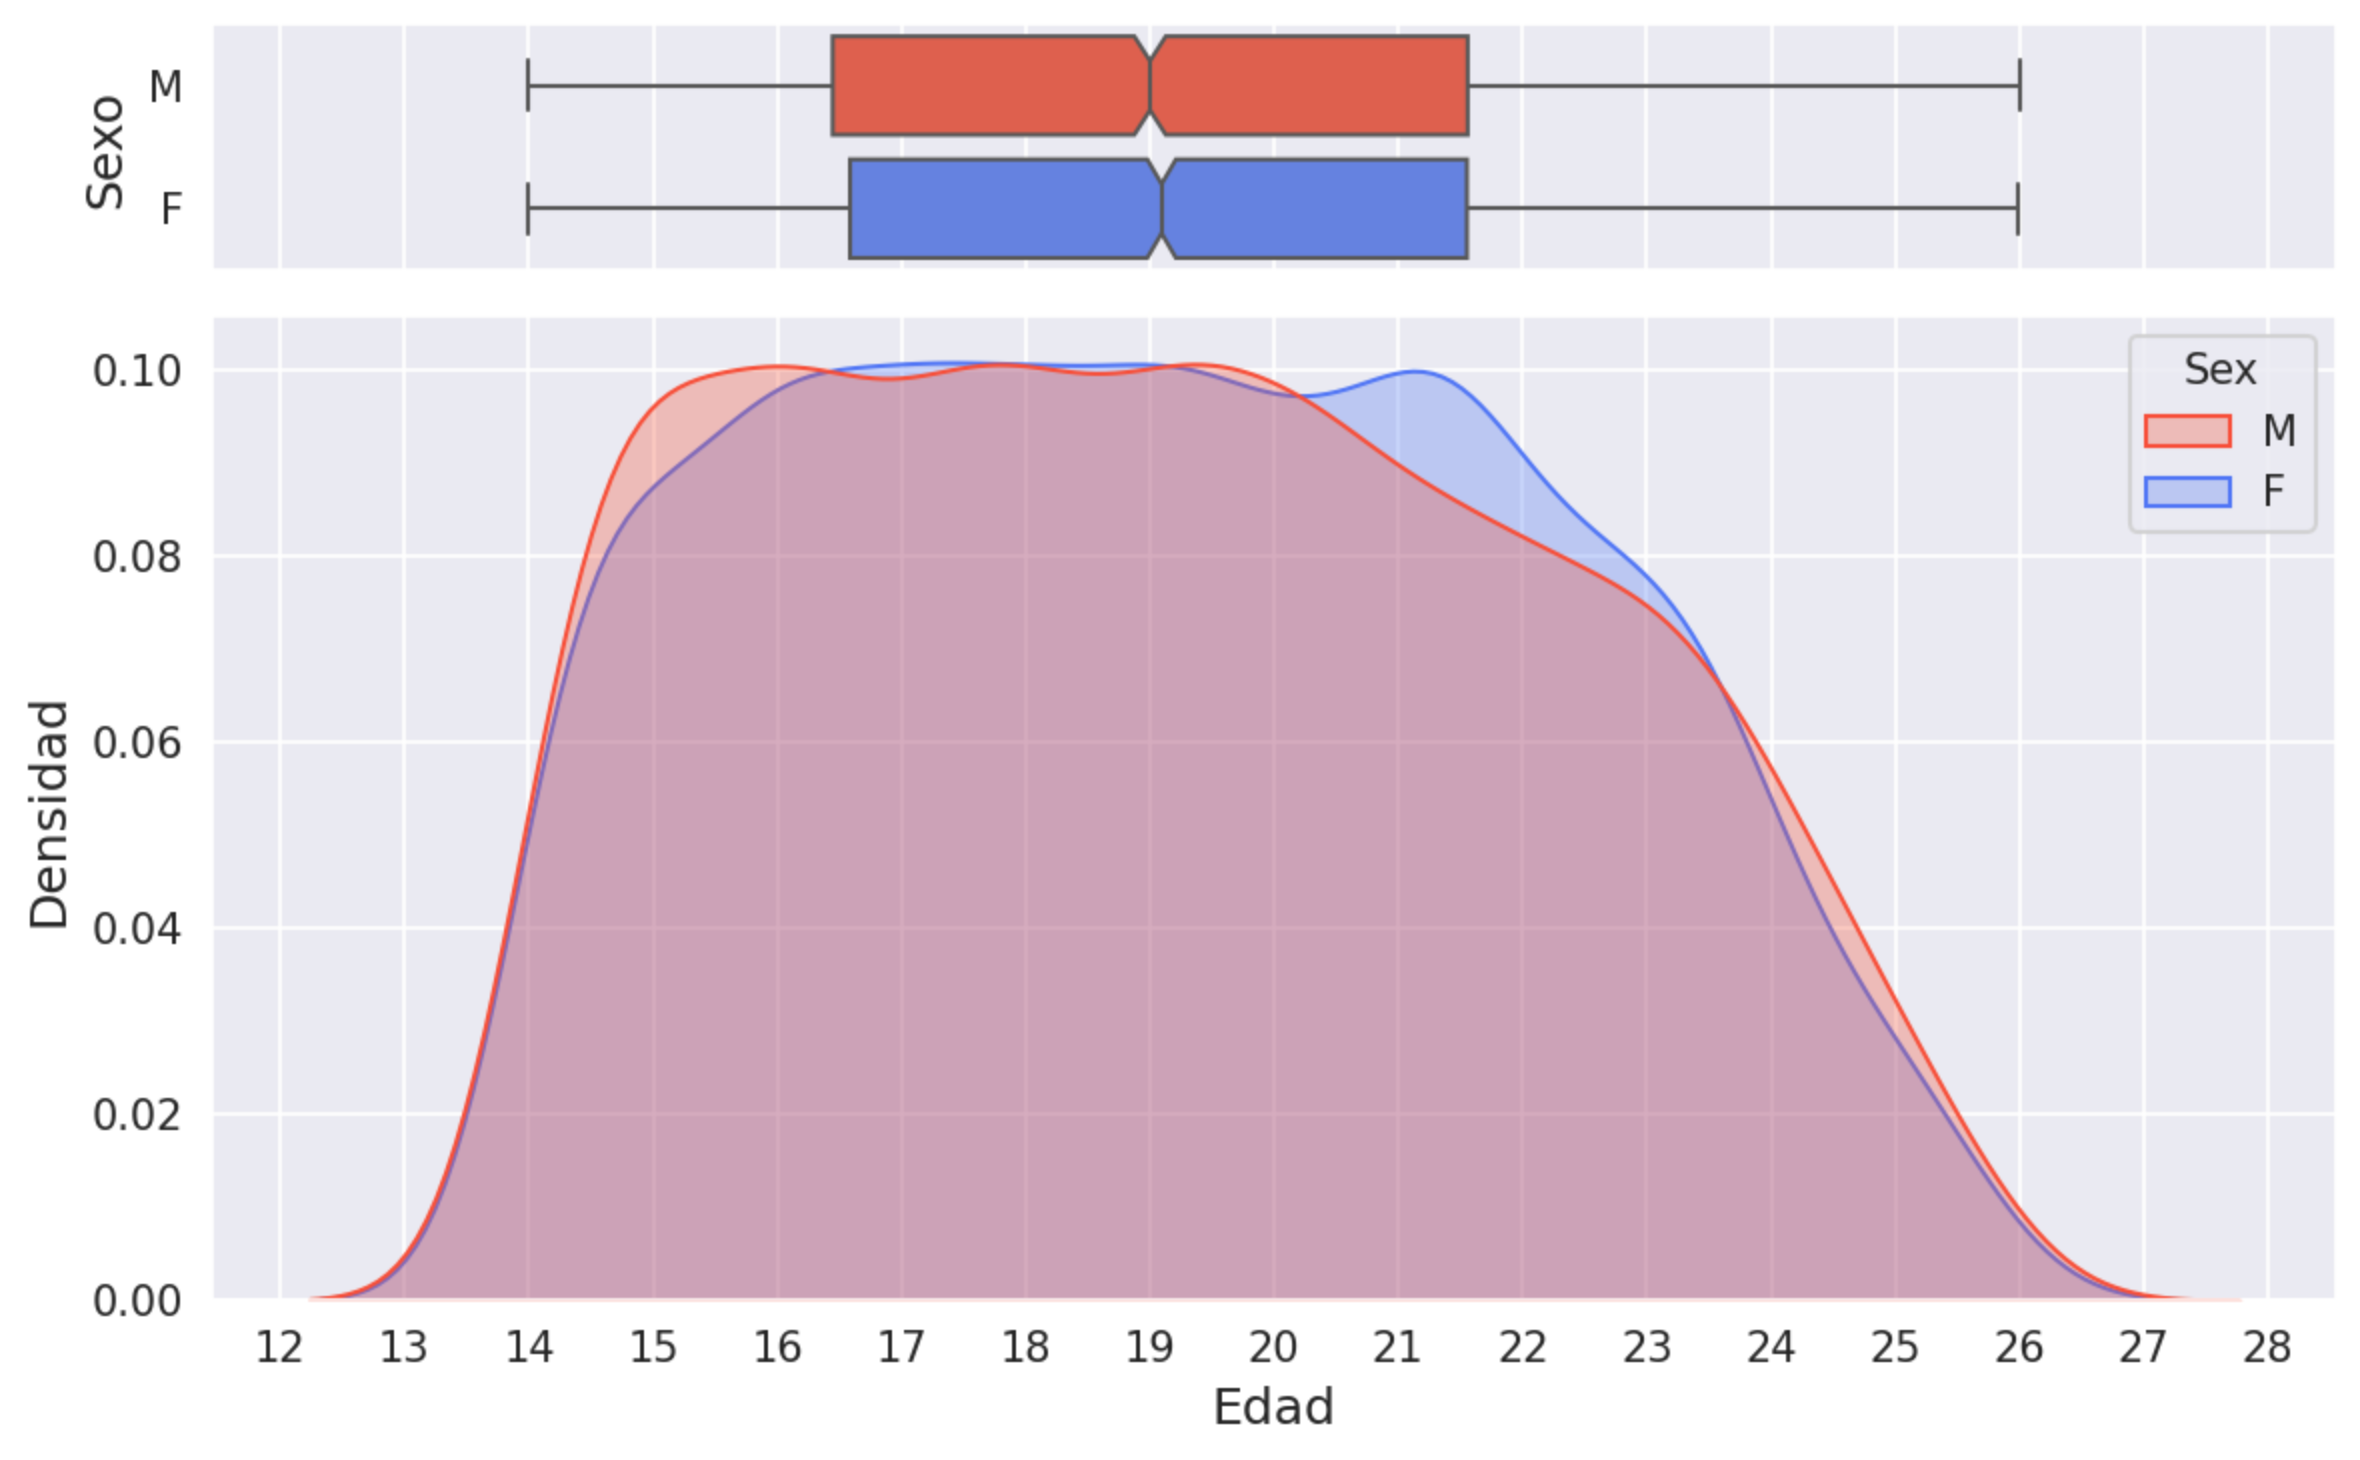
\includegraphics[width=\textwidth]{capitulos/cap_04/imagenes/kdeplot_ages.png}
    \caption[
        Gráficas de densidad y de caja de edad por sexo de los individuos del conjunto de datos disponible.
    ]{
        Gráficas de densidad y de caja de edad por sexo de los individuos del conjunto de datos disponible. 
    } 
    \label{fig:kde_and_boxplot_ages_sex}
\end{figure}

En conclusión, el dataset presenta en general un buen balance entre clases y edades, lo que permite un análisis representativo de la población incluida. No obstante, será necesario examinar con mayor detalle la infrarepresentación de los grupos de mayor edad, especialmente a partir de los 22 años, para evaluar su posible impacto en el rendimiento y generalización de los modelos entrenados.

Se proporcionan los datos ya divididos en \textit{train} ---con un 80\% de los individuos--- y \textit{test} ---con el 20\% restante---, con la intención de que puedan ser utilizados para entrenar y evaluar modelos de predicción. La división de ambos conjuntos se hizo de forma estratificada, de lo que se asume que la distribución será igual en ambos datasets. 

% DATA LEAKAGE:
% En la Figura \ref{fig:kde_ages_train_test} se puede observar cómo existe una distribución 
% edad-sexo similar en los datos de ambos subconjuntos, por lo que se puede asumir que la partición respeta la 
% representatividad de la población original, favoreciendo una evaluación más realista del rendimiento de los 
% modelos en datos no vistos.

% \begin{figure}[h]
%     \centering

%     \begin{subfigure}[b]{0.47\textwidth}
%         \centering
%         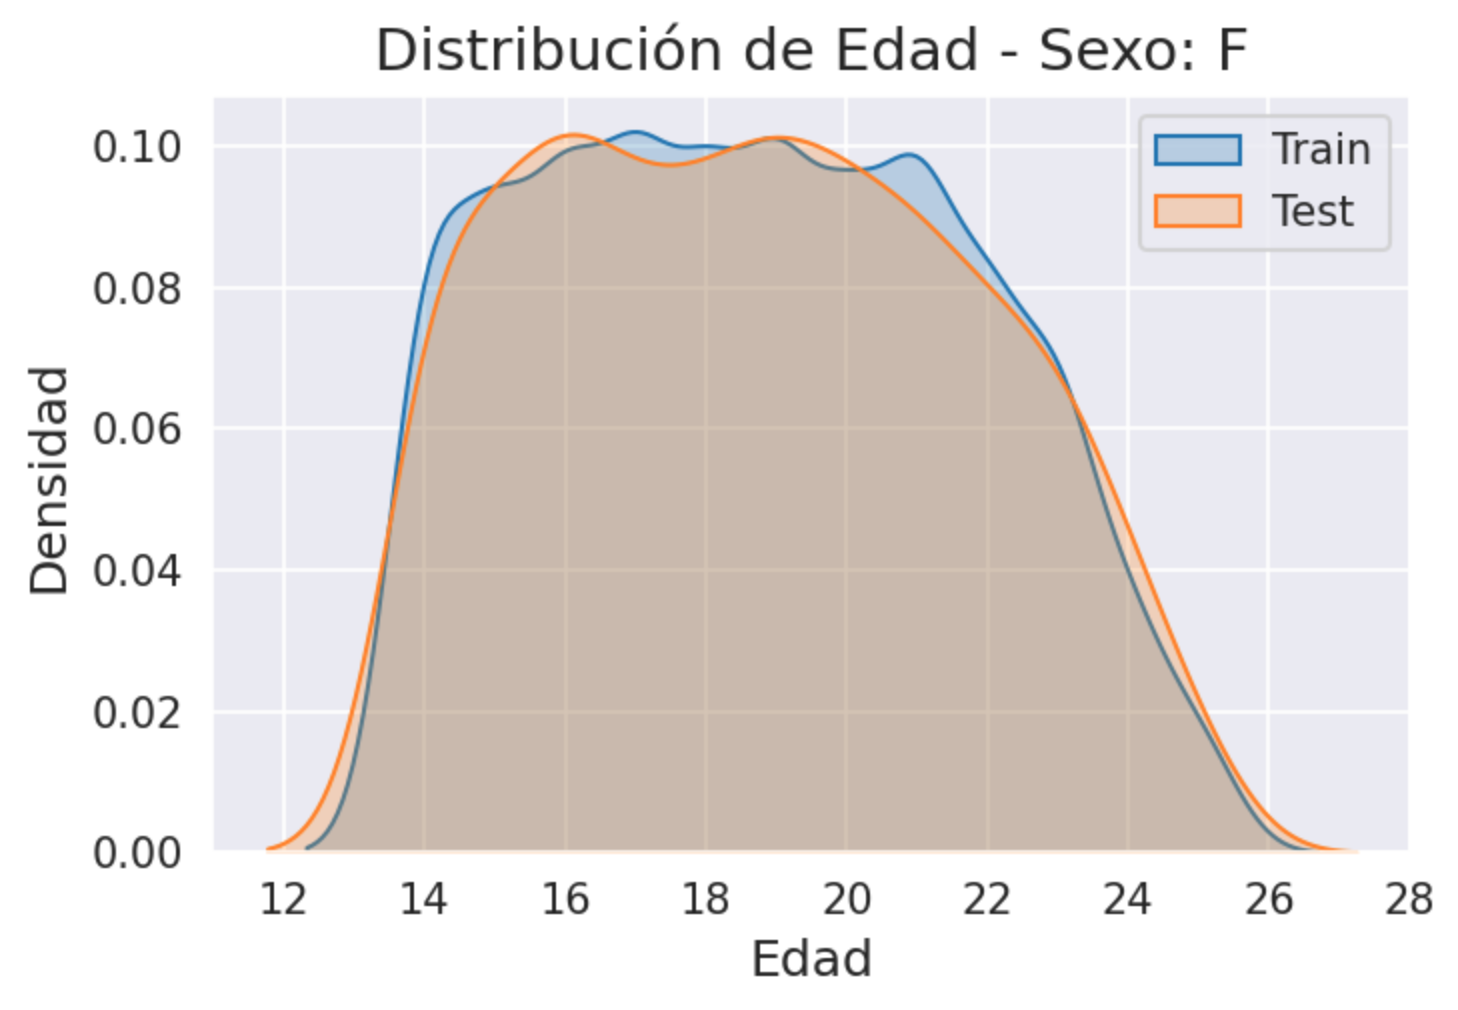
\includegraphics[width=\textwidth]{capitulos/cap_04/imagenes/kde_ages_F.png}
%         \caption{Distribución de edad de individuos de sexo femenino.}
%         \label{fig:kde_ages_F}
%     \end{subfigure}
%     \hfill
%     \begin{subfigure}[b]{0.47\textwidth}
%         \centering
%         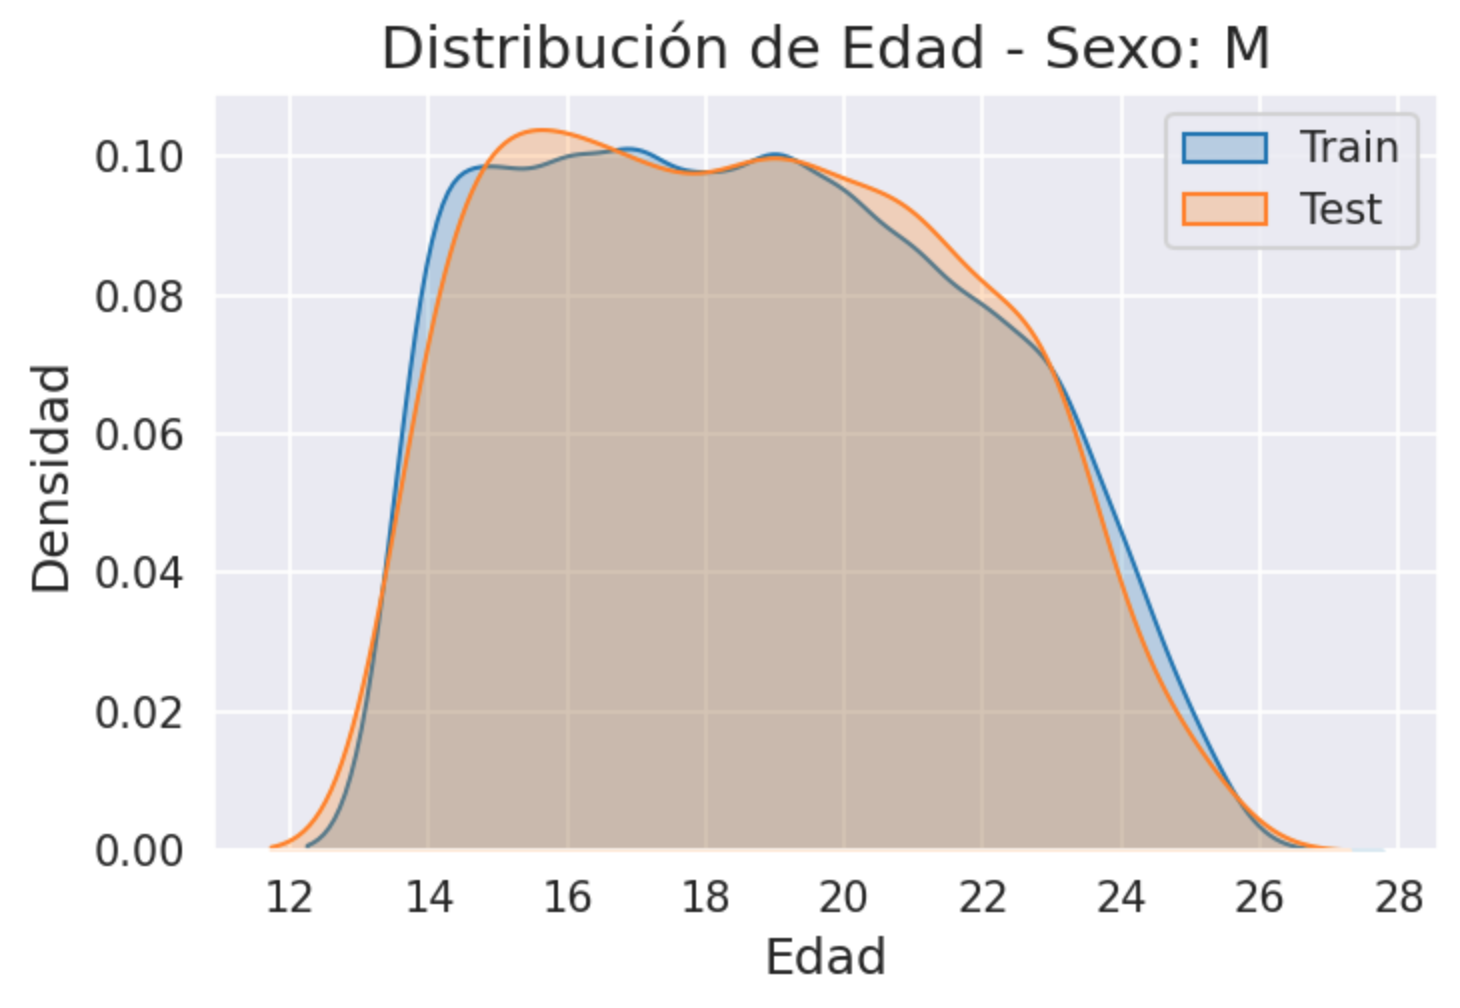
\includegraphics[width=\textwidth]{capitulos/cap_04/imagenes/kde_ages_M.png}
%         \caption{Distribución de edad de individuos de sexo masculino.}
%         \label{fig:kde_ages_M}
%     \end{subfigure}

%     \caption[
%         Distribución de edad de los individuos del conjunto de datos disponible por sexo.
%     ]{
%         Distribución de edad de los individuos del conjunto de datos disponible por sexo. 
%     }
%     \label{fig:kde_ages_train_test}
% \end{figure}


% ------------------------------------------------------------------------------------------------------------
% ------------------------------------------------------------------------------------------------------------

\section{Problemas propuestos}

Como se ha mecionado anteriormente, y con el objetivo de validar los métodos de predicción conformal en diferentes tipos de problemas, este trabajo se centra en tres casuísticas que, si bien están relacionadas en el ámbito de la AF, se tratan de diferente forma en el campo del ML: 

\begin{enumerate}

    \item estimación de la edad legal resuelta como un problema de regresión; 
    
    \item estimación de la edad legal planteada como un problema de clasificación binaria (mayor o menor de 18 años); 
    
    \item estimación de la edad legal resuelta como un problema de clasificación multiclase; y
    
    \item estimación del sexo como problema de clasificación binario.
    
    % \item estimación simultánea de la edad legal y el sexo planteada como un problema de clasificación multiclase, combinando en cuatro clases sexo (masculino o femenino) y la edad (mayor o menor a 18 años).

\end{enumerate}

% ------------------------------------------------------------------------------------------------------------

\subsection{Problema de estimación de edad}

El problema de \textbf{estimación de edad (\textit{age estimation})} consiste en predecir la edad cronológica de un individuo en una escala continua, lo que lo define como un problema de regresión.

Para ello, se ha escogido usar las imágenes de radiografías maxilofaciales como entrada del algoritmo (véase la Figura \ref{fig:regression_problems}). Inicialmente se consideró incluir el sexo como metadato adicional en el modelo; sin embargo, se descartó tras observar de manera preliminar que no tenía un impacto significativo en el rendimiento del modelo, además de que su exclusión simplifica la arquitectura. 

\todo{Para agosto: Un anexo que demuestre esto, yo ya lo he comprobado empíricamente}

\begin{figure}[h]
    \centering
    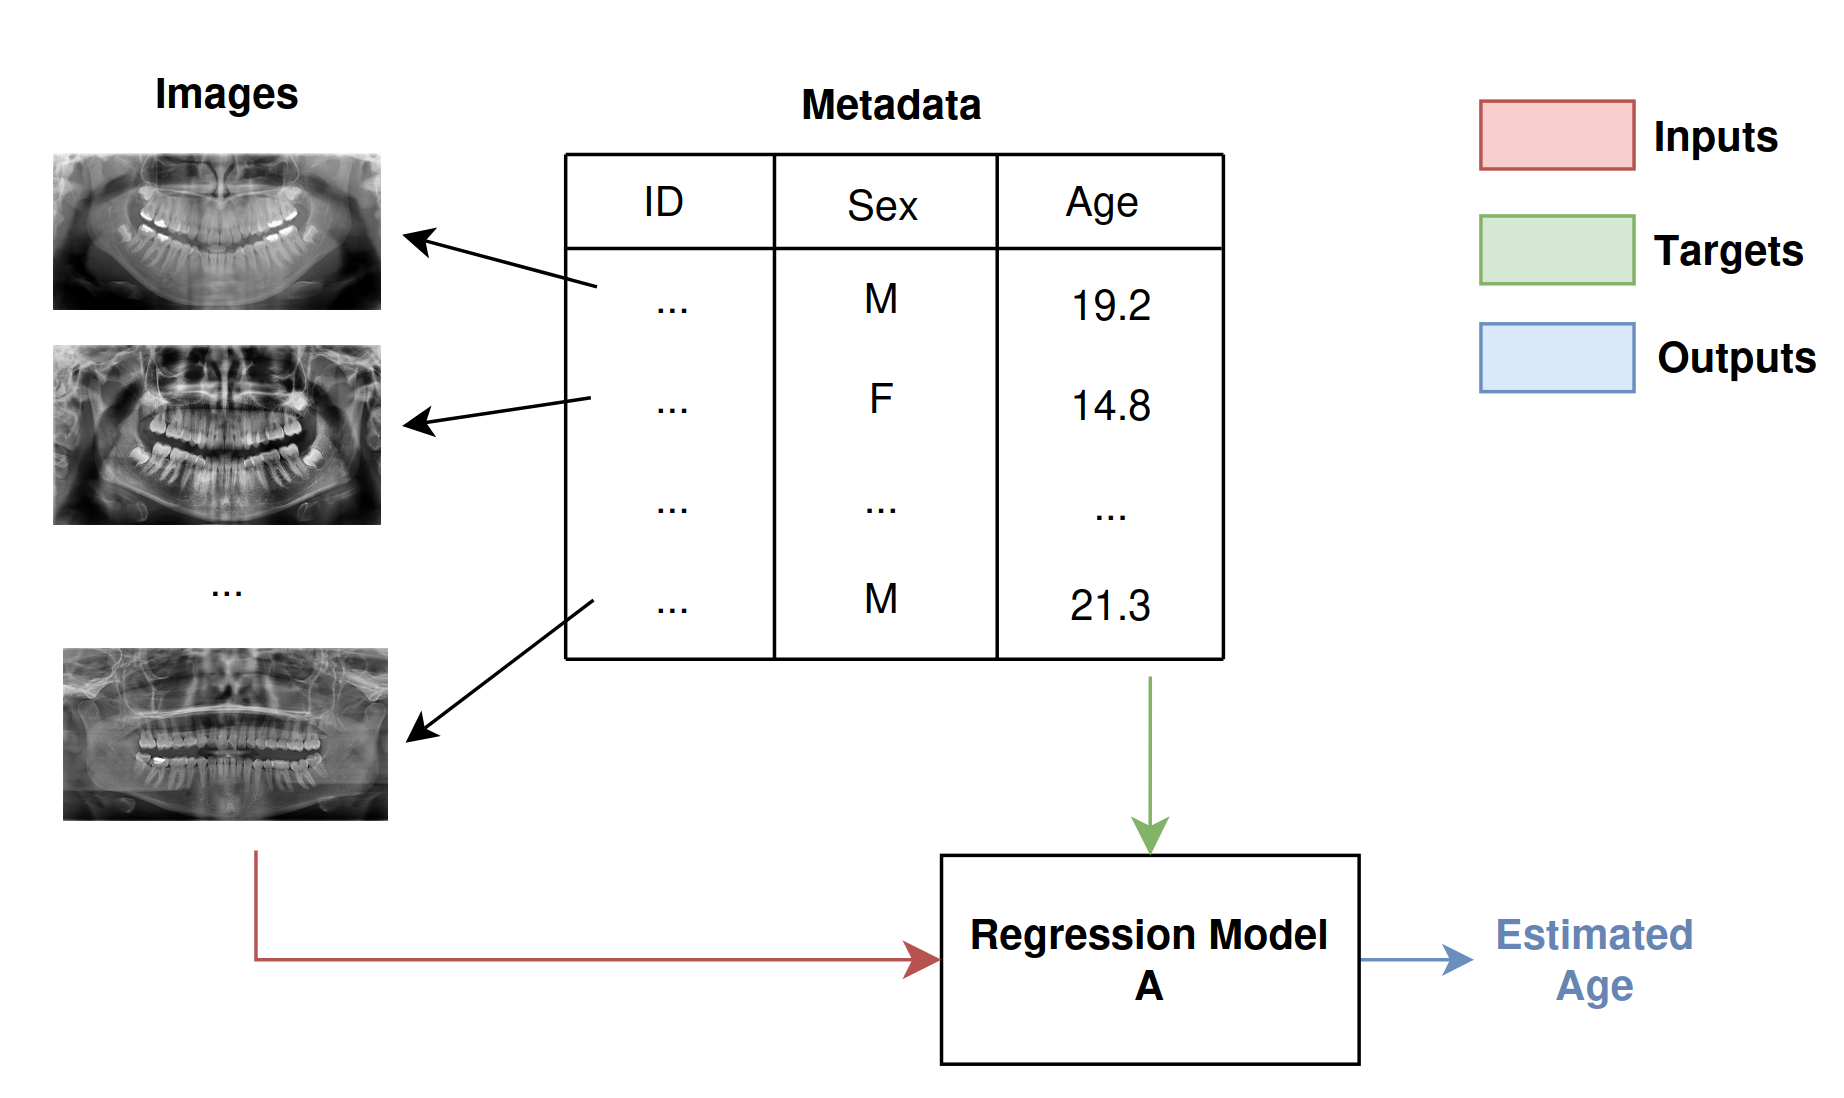
\includegraphics[width=\textwidth]{capitulos/cap_04/imagenes/regression_problem.png}
    \caption[
        Esquema visual del modelos de regresión propuesto. 
    ]{
        Esquema visual del modelos de regresión propuesto. 
        El modelo solo tiene radiografías maxilofaciales como entrada. 
    } 
    \label{fig:regression_problems}
\end{figure}

%ANEXO:Se espera que la información adicional del sexo, como mínimo mantenga el desempeño del modelo, y 
%potencialmente lo mejores, dado que el crecimiento y desarrollo óseo varía entre hombres y mujeres
%\cite{adserias2019, scheuer2000}, lo que sugiere que incluir el sexo como variable de entrada podría ayudar 
%al modelo a ajustar sus predicciones de manera más precisa. 


% ------------------------------------------------------------------------------------------------------------

\subsection{Problema de estimación de mayoría de edad}

Un problema inmediatamente derivado del anterior es la \textbf{clasificación de mayoría de edad (\textit{age majority classification})}, útil en contextos legales donde es necesario determinar si una persona ha alcanzado la mayoría de edad. Este se trata de un problema de clasificación binaria, en el que el objetivo es asignar a cada individuo una de dos clases: ``menor de edad'' o ``mayor de edad''.

\todo{No sé muy bien qué titulo poner para el problema, estoy entre ``clasificación de mayoría de edad'' o ``estimación/valoración de mayoría de edad'' (age assessment). He dejado clasificación para dejar claro que es un problema de este tipo pero en AF se suele usar más bien el segundo término por lo que he podido ver.}


% ------------------------------------------------------------------------------------------------------------

\subsection{Problema de clasificación de edad}

Se propone un problema de estimación de edad, pero planteado como problema de clasificación multiclase, donde cada edad ---como valor entero--- es una clase independiente. 
El potencial para aunar el planteamiento de un problema de regresión con uno de clasificación viene de la mano de la CP, que, aplicada al problema de clasificación, permite generar conjuntos de etiquetas que toleran la cercanía entre clases, de forma que errores pequeños en el valor predicho (por ejemplo, predecir 19 en lugar de 20) no se consideren fallos completos.

% ------------------------------------------------------------------------------------------------------------

% \subsection{Clasificación combinada de mayoría de edad y sexo}

% Finalmente, se propone ampliar el anterior problema a una \textbf{clasificación combinada de mayoría de edad y sexo (\textit{majority age and sex classification})}. Este se trata de un problema de clasificación multiclase, en el que se asigna a cada individuo a una de las posibles combinaciones entre el estatus de mayoría de edad (mayor o menor) y el sexo (masculino o femenino). En total, se consideran cuatro clases: ``menor masculino'', ``menor femenino'', ``mayor masculino'' y ``mayor femenino''.

% Este problema busca evaluar si es posible estimar el sexo de una persona a partir de radiografías maxilofaciales. Para ello, se exploran características morfológicas relevantes, como la forma y tamaño de los caninos \cite{rao1989}, así como los contornos de la rama mandibular y el mentón \cite{indira2012}, cuya morfología presenta una fuerte correlación con el sexo biológico.

% ------------------------------------------------------------------------------------------------------------
% ------------------------------------------------------------------------------------------------------------

\section{Métodos propuestos}

\subsection{Arquitectura empleada}

El primer problema propuesto es el de estimación de edad. Partiremos de un planteamiento muy simple: imágenes bidimensionales de las radiografías panóramicas maxilofaciales ---y sexo, opcionalmente--- como entrada, y estimación de edad a la salida.

Como modelo, empleamos una CNN, dado su buen desempeño en tareas de visión por computador. Específicamente, utilizamos la arquitectura ResNeXt50 \cite{xie2017} preentrenada en Imagenet \cite{deng2009} como punto de partida. Aunque ResNeXt50 fue entrenado originalmente para una tarea de clasificación, se puede adaptar fácilmente a tareas de regresión ---como la estimación de edad--- reemplazando su capa final por una capa de salida adecuada. Por otro lado, a pesar de haber sido entrenado en un dominio diferente al de nuestro problema, el uso de pesos preentrenados ofrece una ventaja significativa: permite una inicialización más robusta que comenzar desde cero, ya que la arquitectura ya ha aprendido a extraer patrones visuales básicos, como bordes y texturas, mediante filtros genéricos.

% ------------------------------------------------------------------------------------------------------------

\subsection{Regresión cuantílica}

La \textbf{regresión cuantílica (\textit{quantile regression}, QR)} es un tipo de regresión que, a diferencia de la regresión puntual, predice intervalos o cuantiles específicos de la distribución de la variable respuesta, en lugar de solo su media. Esta técnica parte de la noción de que la inferencia estadística no se limita a un valor único, sino que puede representarse mediante una distribución de valores probables, de la cual es posible estimar ciertos cuantiles para describir la variabilidad del comportamiento de la variable objetivo.

En este sentido, la regresión cuantílica permite modelar límites inferiores y superiores (por ejemplo, el percentil 10\% y 90\%) para capturar la incertidumbre o heterocedasticidad en los datos. No debe confundirse con una técnica de UQ, ya que no modela explícitamente la incertidumbre epistémica ni proporciona garantías estadísticas de cobertura como lo hacen los métodos de predicción conformal. Sin embargo, puede utilizarse como parte de un enfoque para cuantificar la incertidumbre aleatoria o condicional al estimar intervalos de predicción directamente a partir de los datos.

Esta técnica de regresión puede implementarse en modelos de redes neuronales y modelos tipo \textit{ensemble}, aunque su implementación difiere significativamente. 

En redes neuronales, esta regresión requiere de:

\begin{itemize}

    \item Definir una capa de salida con múltiples neuronas, una por cada cuantil deseado ($\hat{q}_\tau$). Por ejemplo, para obtener una región del 90\% con predicción puntual, tendríamos que inferir los cuantiles 0.05 y 0.95 para los límites inferior y superior, respectivamente, junto con el cuantil 0.5 para la predicción central.

    \item Cambiar la función de pérdida para la estimación de cuantiles. En general, se suele utilizar la pérdida \textit{pinball} \cite{steinwart2011}. La \textbf{función de pérdida \textit{pinball}} es una generalización de la función de pérdida \textit{L1}%
    \footnote{
        También conocida como error absoluto medio, cuantifica la diferencia entre los valores predichos por un modelo y los valores reales como la diferencia absoluta entre cada par:
        
        $$
        L1\textnormal{ loss} = \frac{1}{n} \sum_{i=1}^n |y_i-\hat{y}_i|
        $$
    }, 
    que penaliza las predicciones de manera asimétrica según el error es positivo o negativo. Para un cuantil $\tau \in \left( 0,1\right)$, se define como:

    $$
    L_\tau(y,\hat{q}_\tau) = \left\{
        \begin{array}{rcl}
            \tau \cdot (y-\hat{q}_\tau) & \mbox{si} & y \ge \hat{q}_\tau
            \\
            (1-\tau) \cdot (\hat{q}_\tau-y) & \mbox{si} & y < \hat{q}_\tau
        \end{array}
    \right.
    $$

    La Figura \ref{fig:pinball_loss} ilustra cómo la pérdida penaliza de forma desigual los errores positivos y negativos. Mientras que la pérdida \textit{L1} se centra en ajustar la mediana (cuantil 0.5), la pérdida pinball permite dirigir una salida del modello en cualquier cuantil deseado. Esto es especialmente útil cuando se desea modelar distribuciones asimétricas y capturar diferentes percentiles de la variable de salida, en lugar de asumir una distribución de errores simétrica, como la normal.
    
    A diferencia de con la función de pérdida \textit{L1}, que trata todos los errores como absolutos y busca ajustar la mediana (cuantil 0.5) de la distribución, la \textit{pinball loss} permite enfocar la salida del modelo en cualquier cuantil específico. Esto es especialmente útil para capturar diferentes percentiles de la variable de salida, y modelar la variabilidad en las predicciones de forma más detallada.

    \begin{figure}[h]
        \centering
        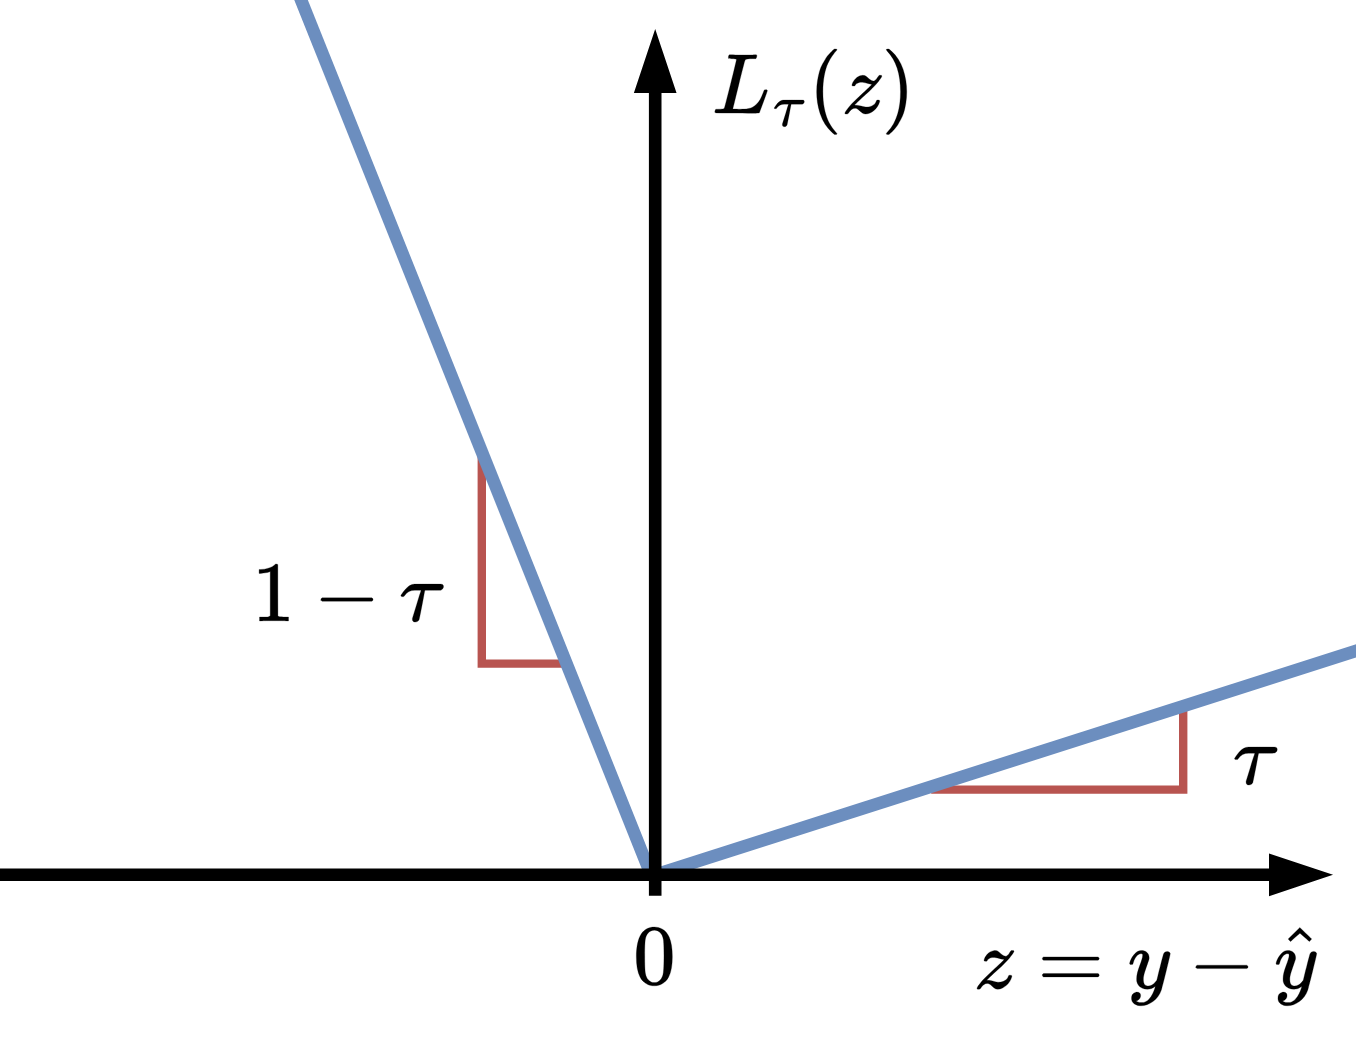
\includegraphics[width=0.5\textwidth]{capitulos/cap_04/imagenes/pinball_loss.png}
        \caption[
            Visualización de la función de pérdida \textit{pinball} para cada valor de error.
        ]{
            Visualización de la función de pérdida \textit{pinball} para cada valor de error.
            Adaptado de la Figura 1 de \cite{romano2019}.
            Esta concretamente muestra la función de pérdida para un cuantil cercano a cero, ya que es más permisivo con los errores positivos que con los negativos, lo cual empujará sus predicciones hacia la parte inferior de la distribución objetivo.
        } 
        \label{fig:pinball_loss}
    \end{figure}

    
    Esta función de pérdida, aplicada a múltiples salidas (cada una asociada a un cuantil específico), busca que las predicciones del modelo cubran la proporción deseada de los datos dentro del intervalo definido por parejas de cuantiles $(\tau_1, \tau_2)$, tratando de cumplir así con un criterio de cobertura probabilística. Por ejemplo: con dos salidas $\tau_1 = 0.05$ y $\tau_2 = 0.95$, se busca que el 90\% las obaservaciones reales ($y$) estén entre los límites predichos de los dos cuantiles ($\hat{q}_{0.05}$ y $\hat{q}_{0.95}$).

    Además, como ya se comentó al inicio, se puede incluir una tercera salida para el cuantil $\tau_3 = 0.5$, correspondiente a la mediana de la distribución condicional, que actúa como una predicción puntual y es equivalente a minimizar la pérdida \textit{L1}.

    Finalmente, el valor arrojado por la función de pérdida conjunta de los cuantiles se suele expresar como la media de las pérdidas para cada cuantil:
    $$
    \mathcal{L}_{total} = \frac{1}{Q} \sum_{i=1}^Q L_{\tau_i} (y, \hat{q}_{\tau_i})
    $$
    donde $Q$ es el número de cuantiles empleados.

\end{itemize}

Por tanto, este tipo de regresión da una estimación puntual $\hat{y}$ (correspondiente a $\hat{q}_{0.5}$) y una estimación interválica formada por límites inferior y superior $\left[ \hat{q}_{lower}, \hat{q}_{upper} \right]$. Este enfoque es ampliamente aplicable y obtiene intervalos adaptativos a la heterocedasticidad de los datos \cite{romano2019}. Sin embargo, no tiene garantías estadísticas de cobertura bajo distribuciones arbitrarias de errores. Es por ello que se requiere de herramientas adicionales para garantizar la cobertura.

% ------------------------------------------------------------------------------------------------------------

\subsection{Métodos de predicción conformal para regresión}

Todos los métodos propuestos en este trabajo son \textit{split calibration}, es decir, los datos de entrenamiento se dividen en dos subconjuntos: entrenamiento y calibración. No hemos implementado métodos \textit{cross-calibration} como \cite{barber2021} dado que requieren un mayor coste computacional. Además, en los experimentos preliminares, \textit{split calibration} demostró ser suficiente para obtener valores razonablemente buenos de cobertura marginal y una eficiencia adecuada en los intervalos de predicción.

% ------------------------------------------------------------------------------------------------------------

\subsubsection{\textit{Inductive Conformal Prediction} (ICP)}

La ICP \cite{papadopoulos2002} fue el primer método de predicción conformal desarrollada para problemas de regresión. Su planteamiento es muy simple: consiste en añadir un margen a las predicciones puntuales, calculado a partir de un cuantil del error absoluto observado en un conjunto de calibración independiente. Este margen permite construir intervalos de predicción que contienen el valor real con una probabilidad determinada previamente (por ejemplo, 90\% o 95\%). 

Por ello, la función de no conformidad es el error absoluto de la predicción respecto al valor real:

$$
A(x_i, y_i) = | y_i - \hat{f}(x_i) |
% R = \left\{ | y_i - \hat{f}(x_i) | \right\}_{i=1,...,n}
$$

Luego, el umbral de no conformidad para un nivel de confianza $1-\alpha$ se calcula como el cuantil $(1-\alpha)(1+1/n)$ de las puntuaciones de no conformidad:

$$
\delta_\alpha = Quantile_{ \lceil  (1-\alpha) (1 + 1/n)  \rceil } ( \left\{ A(x_i,y_i) \right\}_{i=1}^n )
$$

Finalmente, para una instancia $x_{n+1}$, el intervalo de predicción $C(x_{n+1})$ se construye como: 

$$
\hat{C_\alpha}(x_{n+1}) = \left[ \hat{f}(x_{n+1}) - \delta_\alpha, \hat{f}(x_{n+1}) + \delta_\alpha\right]
$$

Este método de CP presenta varias ventajas: 

\begin{itemize}

    \item \textbf{\textit{Model-agnostic} y \textit{domain-agnostic}}: Es independiente tanto del modelo como del dominio, ya que no utiliza representaciones internas del modelo ni de las entradas. 
    
    \item \textbf{Bajo coste computacional}: Solo añade coste computacional en la calibración, con el cálculo de puntuaciones de no conformidad en calibración $\left( \mathcal{O}(n_{calib}) \right)$ y cálculo del umbral de no conformidad $\left( \mathcal{O}(n_{calib} \log n_{calib}) \right)$. La inferencia conformal mantiene el mismo orden de coste que el modelo base ($\mathcal{O}(1)$ por predicción). 

\end{itemize}

Sin embargo, también presenta importantes limitaciones: 

\begin{itemize}
    
    \item \textbf{Intervalo simétrico y no adaptativo}: El intervalo es simétrico, además de tener siempre el mismo ancho ($2q_{1-\alpha}$), no permitiendo adaptarse a la incertidumbre específica de cada predicción. 

    \item \textbf{Sensibilidad a datos ruidosos o OOD}: Si el conjunto de calibración contiene \textit{outliers} o viola el supuesto de intercambiabilidad, el umbral \(q_{1-\alpha}\) puede inflarse, generando intervalos excesivamente conservadores. Tampoco detecta heterocedasticidad automáticamente.

\end{itemize}

% ------------------------------------------------------------------------------------------------------------

\subsubsection{\textit{Conformalized Quantile Regression} (CQR)}

Como su nombre indica, este método se realiza sobre la regresión cuantílica. La CQR \cite{romano2019} combina la flexibilidad de la regresión cuantílica para estimar directamente los cuantiles condicionales con la garantía de validez estadística proporcionada por la conformalización. Esto permite obtener intervalos de predicción que son asimétricos y adaptativos, ajustándose localmente a la variabilidad y distribución de los datos.

Se ha optado por implementar la segunda definición del intervalo de predicción, presentada en el segundo teorema de \cite{romano2019}, que incluye la calibración de ambas colas para obtener intervalos asimétricos \cite{linusson2014}. Según el artículo, esta opción mejora las garantías de cobertura, aunque puede implicar un aumento en el ancho del intervalo.

El proceso de calibración de este método se lleva a cabo de la siguiente manera: 

\begin{itemize}
    \item Se calculan las puntuaciones de no conformidad sobre los datos del conjunto de calibración como las diferencias entre los valores observados y los límites del intervalo predictivo:
    
    \begin{equation*}
    \begin{split}
        A_{lower}(x_i,y_i) = \hat{q}_{lower}(x_i) - y_i \\
        A_{upper}(x_i,y_i) = y_i - \hat{q}_{upper}(x_i)  
    \end{split}
    \end{equation*}

    donde $\hat{q}_{upper}(x_i)$ y $\hat{q}_{lower}(x_i)$ representan los límites superior e inferior del intervalo predictivo para la observación $x_i$, respectivamente, e $y_i$ es el valor observado real.

    \item Se calcula un umbral de no conformidad para un nivel de confianza dado $1-\alpha$ como el cuantil $(1-\alpha)(1+1/n)$ de $R$:

    \begin{equation*}
    \begin{split}
        \delta_{lower_\alpha} &= Quantile_{ \lceil  (1-\alpha) (1 + 1/n)  \rceil } ( \left\{ A_{lower}(x_i,y_i) \right\}_{i=1}^n  ) \\
        \delta_{upper_\alpha} &= Quantile_{ \lceil  (1-\alpha) (1 + 1/n)  \rceil } ( \left\{ A_{upper}(x_i,y_i) \right\}_{i=1}^n  )
    \end{split}
    \end{equation*}

\end{itemize}

Tras haber calibrado el modelo, para una instancia $x_{n+1}$, el intervalo de predicción $C(x_{n+1})$ se
construye como:

$$
\hat{C_\alpha}(x_{n+1}) = 
        \left[ 
            \hat{q}_{lower}(x_{n+1}) - \delta_{lower_\alpha}, 
            \hat{q}_{upper}(x_{n+1}) + \delta_{upper_\alpha}
        \right]
$$

CQR, al igual que ICP, es independiente del modelo y del dominio, ya que solo emplea las salidas y valores reales para realizar la calibración. También tiene el mismo orden de eficiencia computacional, puesto que realiza prácticamente las mismas operaciones que ICP, pero para cada límite del intervalo predicho, calibrando los cuantiles inferior y superior de manera independiente para mantener la cobertura deseada.

Sin embargo, CQR logra intervalos asimétricos y adaptativos, dado que la regresión cuantílica estima directamente los cuantiles condicionales de la distribución de la variable objetivo, permitiendo que los límites del intervalo se ajusten según la heterocedasticidad y la forma local de la distribución de los datos, en lugar de asumir una distribución simétrica o constante del error. 

En la Tabla \ref{tab:comparativa_cp} observamos un cuadro comparativo de los distintos métodos propuestos de CP. 

\renewcommand{\arraystretch}{1.5}
\begin{sidewaystable}
    \centering
    \begin{tabular}{lllll}
    \hline
    Característica                                                               & base                  & ICP            & QR                    & CQR                                                                      \\ \hline
    \begin{tabular}[c]{@{}l@{}}Cobertura \\ Marginal\end{tabular}                & No garantizada        & Garantizada    & No garantizada        & Garantizada                                                              \\
    \begin{tabular}[c]{@{}l@{}}Cobertura \\ Condicionada\end{tabular}            & No garantizada        & No garantizada & No garantizada        & \begin{tabular}[c]{@{}l@{}}No garantizada, \\ pero aproxima\end{tabular} \\
    Model-agnostic                                                               & Sí                    & Sí             & Sí                    & Sí                                                                       \\
    Domain-agnostic                                                              & Sí                    & Sí             & Sí                    & Sí                                                                       \\
    \begin{tabular}[c]{@{}l@{}}Intervalos \\ simétricos/asimétricos\end{tabular} & Simétricos            & Simétricos     & Asimétricos           & Asimétricos                                                              \\
    Intervalos adaptativos                                                       & No                    & No             & Sí                    & Sí                                                                       \\
    Coste calibración                                                            & No existe calibración & O(n log(n))    & No existe calibración & O(n log(n))                                                              \\
    \begin{tabular}[c]{@{}l@{}}Coste inferencia \\ (por predicción)\end{tabular} & O(1)                  & O(1)           & O(1)                  & O(1)                                                                     \\ \hline
    \end{tabular}
    \caption[
        Comparativa de métodos propuestos de CP para problemas de regresión.
    ]{   
        Comparativa de métodos propuestos de CP para problemas de regresión.
    }
    \label{tab:comparativa_cp}
\end{sidewaystable}

% ------------------------------------------------------------------------------------------------------------
% ------------------------------------------------------------------------------------------------------------

\subsection{Calibración de probabilidades en clasificación}

\todo{Hacer este apartado. No debería ser muy largo. Presentar solo el método de Platt Scaling.}

% ------------------------------------------------------------------------------------------------------------
% ------------------------------------------------------------------------------------------------------------

\subsection{Métodos de predicción conformal para clasificación}

\subsubsection{\textit{Least-Ambiguous set-valued Classifiers} (LAC)}

LAC \cite{sadinle2019} es el primer método propuesto de predicción conformal para problemas de clasificación. Propone un enfoque de clasificación de conjuntos de valores (\textit{set-valued classification}) en el que, en lugar de asignar una única etiqueta a cada instancia, se selecciona un conjunto de etiquetas que garanticen un nivel de confianza predeterminada por el usuario.

La función de no conformidad es conocida como \textbf{probabilidad inversa o \textit{hinge loss}} \cite{johansson2017}, y se calcula como la unidad menos la probabilidad de la clase verdadera%
\footnote{
    Se le denomina probabilidad a un valor de certeza que realmente no tiene garantías estadísticas, ya que proviene directamente de la salida \textit{softmax} o sigmoide del modelo. Estas salidas no están necesariamente bien calibradas ni corresponden a verdaderas probabilidades, si bien el término se utiliza frecuentemente por motivos de simplicidad y comunicación.
}
o, lo que es lo mismo, la suma de valores de probabilidad de todas las clases salvo la correspondiente a la etiqueta verdadera:
$$
A(x_i,y_i) = 1- \hat{\pi}_{y_i}(x_i)
$$

donde $\hat{\pi}_{y_i}(x_i)$ es la probabilidad para la clase de la etiqueta verdadera%
\footnote{
    $\hat{\pi}(x_i)$ es el vector de probabilidades de las clases para la instancia $i$.
}.


El umbral de no conformidad para un nivel de confianza $1-\alpha$ se calcula como el cuantil 
$(1-\alpha)(1+1/n)$ de las puntuaciones de no conformidad:

$$
\delta_\alpha = Quantile_{ \lceil  (1-\alpha) (1 + 1/n)  \rceil } ( \left\{ A(x_i,y_i) \right\}_{i=1}^n)
$$

El conjunto de predicción conformal de una nueva instancia $x_{n+1}$ se construye como las clases cuyas probabilidades superan la unidad menos el umbral de no conformidad:

$$
\Gamma_\alpha(x_{n+1}) = \left\{ k | \hat{\pi}_k(x_{n+1}) \ge 1-\delta_\alpha \right\} 
$$

Así, se seleccionan aquellas clases cuya probabilidad es lo suficientemente alta como para superar el umbral de no conformidad previamente calculado. No obstante, puede ocurrir que, para ciertas instancias, ninguna clase alcance dicho umbral, lo que resultaría en un conjunto de predicción vacío. Para evitar esta situación, se ha optado por incluir en estos casos todas las clases posibles dentro del conjunto de predicción. Esta elección responde a una estrategia conservadora: ante la falta de evidencia suficiente para respaldar alguna clase en particular con el nivel de confianza requerido, lo más prudente es no excluir ninguna posibilidad, y así reflejar una alta incertidumbre. 

Algunas propiedades de este método son:

\begin{itemize}

    \item \textbf{\textit{Model agnostic}}: Es independiente del modelo, ya que solo necesita el vector de puntuaciones predictivas $\hat{\pi}(x_i)$ y la etiqueta verdadera para cada instancia $y_i$.  

    \item \textbf{Conjuntos de predicción no adaptativos}: A pesar de poder presentar conjuntos con distinto número de clases predichas, emplea un único umbral calibrado globalmente sobre todas las muestras y clases por igual. 

    \item \textbf{Bajo coste computacional}: Solo añade coste computacional en la calibración, con el cálculo de puntuaciones de no conformidad ($\mathcal{O}(n_{calib})$) y la obtención del umbral de no conformidad ($\mathcal{O}(n_{calib})log n_{calib}$). No añade coste a la inferencia ($\mathcal{O}(1)$).
    
\end{itemize}

\todo{Falta añadir una imagen que refleje la intuición detrás de esta técnica}

% ------------------------------------------------------------------------------------------------------------

\subsubsection{Mondrian Confidence Machine (MCM)}

(MCM) \cite{vovk2003} es un método estrechamente relacionado con LAC, ya que emplea el mismo esquema general de CP. Sin embargo, introduce una diferencia clave: en lugar de aplicar un único umbral global para todas las clases, MCM segmenta el conjunto de calibración por clase y calcula las puntuaciones de no conformidad y los umbrales de decisión de forma independiente para cada una.

A continuación, se detallan sus principales característica diferenciadas de LAC:

\begin{itemize}

    \item \textbf{Garantiza cobertura condicional por clase}, lo cual es muy útil en conjuntos desbalanceados. A diferencia de LAC, que ofrece cobertura marginal sobre el conjunto total, MCM busca asegurar que cada clase individual cumpla el nivel de cobertura deseado, lo que favorece una distribución más equitativa del error.
    
    \item \textbf{Conjuntos de predicción parcialmente adaptativos}: Estos son adaptativos respecto a cada clase, aunque no por muestra, ya que emplea un umbral de no conformidad por cada clase, pero los aplica igual a todas las muestras.  

    \item \textbf{Coste computacional ligeramente superior a LAC}: En la calibración, se requiere calcular las puntuaciones de no conformidad y el umbral de no conformidad para cada clase, lo cual puede aumentar los tiempos linealmente en base al número de clases. La inferencia sigue manteniendo la eficiencia. No obstante, sigue siendo un método eficiente y apto para entornos de predicción en tiempo real, siempre que el número de clases no sea excesivo.

\end{itemize}

% ------------------------------------------------------------------------------------------------------------

\subsubsection{Adaptive Prediction Sets (APS)}

APS \cite{romano2020}, como sugiere su nombre, tiene como objetivo generar conjuntos de predicción adaptativos, cuyo tamaño se ajusta dinámicamente en función de la incertidumbre del modelo para cada muestra. De este modo, se busca que las predicciones sean más informativas y reflejen con mayor precisión la confianza del modelo.

La función de no conformidad utilizada en APS evalúa, para cada instancia, la probabilidad total acumulada en aquellas clases que el modelo considera al menos tan probables como la clase verdadera. En otras palabras, se calcula como la suma de las probabilidades predichas para todas las clases cuya probabilidad es mayor o igual a la asignada a la etiqueta correcta.

Sea el vector $\hat{\pi}$ ordenado en orden decreciente: 
$$
\hat{\pi}_{(1)}(x_i) \ge \hat{\pi}_{(2)}(x_i) \ge \cdot\cdot\cdot \ge \hat{\pi}_{(K)}(x)
$$
donde $(k)$ es el índice de la clase con la $k$ mayor probabilidad, la función de no conformidad se define como:
$$
A(x_i, y_i) = \sum_{j=1}^k \hat{\pi}_{(j)}(x_i) \textnormal{ donde } (k)=y_i 
% R = \left\{ \sum_{j=1}^k \hat{\pi}_{(j)}(x_i)  \right\}_{i=1,...,n} \textnormal{ donde } (k)=y_i
$$

Cabe destacar que, en el caso particular de clasificación binaria, esta medida de no conformidad coincide exactamente con la utilizada en el método LAC, ya que la acumulación se limita a una o dos clases. Por tanto, ambos métodos resultan equivalentes en este escenario. Sin embargo, divergen en problemas multiclase, donde las puntuaciones de no conformidad de APS son más permisivas que las de LAC, ya que reconocen que un modelo puede identificar características comunes entre varias clases y generar valores probabilísticos repartidos. No existe incertidumbre cuando la puntuación probabilística más alta corresponde a la clase verdadera. Por tanto, APS penaliza menos los casos en que la clase correcta está entre las más probables, aunque no necesariamente en primer lugar.

A partir de las puntuaciones de no conformidad en el conjunto de calibración, se calcula el umbral de no conformidad de la manera habitual:

$$
\delta_\alpha = Quantile_{ \lceil  (1-\alpha) (1 + 1/n)  \rceil } ( \left\{ A(x_i,y_i) \right\}_{i=1}^n )
$$

Tras la calibración, para una nueva instancia $x_{n+1}$, se calcula la distribución de probabilidad ordenada en orden decreciente, y se suman de forma acumulada las probabilidades desde la clase más probable hasta que dicha suma sea mayor o igual que el umbral calibrado. El conjunto de predicción $\Gamma_\alpha(x_{n+1})$ se forma entonces incluye todas las clases correspondientes a ese conjunto acumulado: 

$$
\Gamma_\alpha(x_{n+1}) = \left\{ (1),...,(k) \right\} \\ \textnormal{ donde } 
k = min\left\{ j: \sum_{i=1}^{j} \hat{\pi}_{(i)}(x_{n+1}) \ge \delta_\alpha \right\} 
$$

Este algoritmo, al igual que LAC, solo garantiza cobertura marginal, pero genera \textbf{conjuntos de predicción más adaptativos} respecto a la incertidumbre inherente a la predicción de cada instancia. A diferencia de métodos con umbrales fijos, ajusta dinámicamente el tamaño de los conjuntos según la confianza del modelo en regiones específicas del espacio de características.

Sin embargo, en la práctica se ha observado que esta adaptabilidad conlleva \textbf{conjuntos de predicción más grandes en promedio} \cite{romano2020, angelopoulos2020}. Este fenómeno es un \textit{trade-off} inherente al intentar \textbf{aproximar la cobertura condicional} sin asumir distribuciones subyacente, que analizaremos en profundidad con nuestros datos en la experimentación. 

% ------------------------------------------------------------------------------------------------------------

\subsubsection{Regularized Adaptive Prediction Sets (RAPS)}

RAPS \cite{angelopoulos2020} es una variante del método APS, que introduce modificaciones clave para reducir el tamaño de los conjuntos de predicción, especialmente en escenarios con muchas clases, donde APS tiende a generar conjuntos excesivamente grandes. El objetivo principal de RAPS es mantener la propiedad de cobertura marginal deseada, al tiempo que se obtienen conjuntos de predicción más compactos y útiles en la práctica. 

RAPS extiende la función de no conformidad utilizada en APS mediante la incorporación de un término de regularización que penaliza explícitamente la inclusión de clases con baja probabilidad en conjuntos de predicciones de tamaño ya elevado. 

Para ello, se introducen dos hiperparámetros en la función de no conformidad:

\begin{itemize}

    \item $k_{reg}$ representa el tamaño mínimo del conjunto de predicción a partir del cual se comenzará a aplicar penalización. Es decir, los conjuntos de predicción de tamaño menor o igual a $k_{reg}$ no serán penalizados, ya que se asume que, si todos los conjuntos tuvieran como máximo ese tamaño, la cobertura marginal aún se mantendría. 
    
    El valor de este hiperparámetro se determina empíricamente observando, en el conjunto de calibración, cuál es el menor tamaño de conjunto que cumple con la cobertura deseada en una fracción suficientemente alta de las instancias. 
   
    \item $\lambda$, un parámetro de regularización que penalizará más a aquellos conjuntos que superen $k_{reg}$ etiquetas predichas cuanto mayor número de etiquetas tengan. 

    Este hiperparámetro se determina típicamente a través de validación en un conjunto de datos independiente al de calibración, mediante búsqueda de hiperparámetros que minimicen el tamaño medio del conjunto de predicción sin comprometer significativamente la cobertura marginal. En la práctica, se suele probar con varios valores posibles para $\lambda$ y seleccionar el que logre el mejor equilibrio entre concisión y cobertura en el conjunto de validación.

\end{itemize}

Una vez determinados los valores de estos hiperparámetros, se calculan las puntuaciones de no conformidad de la siguiente manera:

$$
A(x_i, y_i) = \sum_{j=1}^k \hat{\pi}_{(j)}(x_i) + \lambda (k-k_{reg})^+ \textnormal{ donde } (k) = y_i
$$

El procedimiento de calibración y predicción en RAPS sigue la misma estructura general que APS, pero utiliza la función de no conformidad regularizada en lugar de la acumulación pura de probabilidades. Así, el umbral calibrado se calcula como:

$$
\delta_\alpha = Quantile_{ \lceil  (1-\alpha) (1 + 1/n)  \rceil } \left( \left\{ A(x_i,y_i) \right\}_{i=1}^n \right)
$$

Y el conjunto de predicción para una nueva instancia $x_{n+1}$ se construye como

$$
\Gamma_\alpha(x_{n+1})= \left\{ (1), ..., (k) \right\} \textnormal{ donde } k = min\left\{ j: \sum_{i=1}^{j} \pi_{(i)}(x_{n+1}) + \lambda (k-k_{reg})^+  \ge \delta_\alpha \right\}
$$

Gracias a la regularización, RAPS tiende a generar conjuntos de predicción más pequeños que APS, especialmente cuando la clase verdadera se encuentra entre las más probables (y por tanto el hiperparámetro $k_{reg}$ tiene un valor bajo).

% ------------------------------------------------------------------------------------------------------------

\subsubsection{Sorted Adaptive Prediction Sets (SAPS)}

SAPS \cite{huang2023conformal} propone un enfoque distinto a métodos previos como APS y RAPS. Los autores identifican una limitación importante en estos algoritmos: las probabilidades producidas por la capa \textit{softmax} suelen seguir una distribución con cola larga, lo que facilita la inclusión de clases poco probables en los conjuntos de predicción. Esto lleva a la generación de conjuntos innecesariamente grandes, que reducen la utilidad práctica del método.

SAPS argumenta que muchas de estas probabilidades de baja magnitud representan información redundante o poco útil para la tarea de predicción conforme. En lugar de utilizar todo el vector de probabilidades, propone construir los conjuntos de predicción únicamente a partir de dos elementos clave: 
\begin{itemize}
    \item la probabilidad más alta (asociada a la clase predicha como más probable), y
    \item el orden de clasificación de las clases según el modelo.
\end{itemize}

A partir de esta representación reducida, SAPS ordena las clases por probabilidad decreciente y aplica un esquema adaptativo de umbral basado en la posición en el ranking, en lugar de en el valor absoluto de la probabilidad. De esta forma, se evita el efecto negativo de las colas largas y se prioriza la inclusión de clases con mayor relevancia relativa según el modelo.




\todo{Por completar (JULIO)}

Al enfocarse en esta información comprimida y más representativa, SAPS logra generar conjuntos más compactos, sin comprometer la garantía de cobertura estadística que exige el marco de predicción conforme.





Primero, en su planteamiento, y a diferencia de los métodos anteriores, no define una métrica de no conformidad, sino más bien una métrica de confianza, 



% ------------------------------------------------------------------------------------------------------------
% ------------------------------------------------------------------------------------------------------------

\section{Métricas}


\subsection{Métricas para regresión}

En nuestro problema de regresión emplearemos dos tipos de métricas con el objetivo de evaluar aspectos distintos del desempeño del modelo.

Por una parte, las métricas destinadas a las predicciones puntuales se basan fundamentalmente en medir el error entre el valor real ($y_i$) y el valor esperado predicho ($\hat{y_i}$). Estas métricas nos permiten cuantificar directamente la discrepancia entre las estimaciones del modelo (estimación central en modelos de predicción interválica) y la \textit{ground truth}. Las métricas que empleamos para estas predicciones son:

\begin{itemize}
    \item El \textbf{error absoluto medio (\textit{mean absolute error}, MAE)} mide el promedio de las diferencias absolutas entre los valores reales ($Y_i$) y los valores predichos ($\hat{Y_i}$) por el modelo.

    $$
    MAE = \frac{1}{n} \sum_{i=1}^n{|y_i - \hat{y_i}|} \in [0, \infty)
    $$

    donde $n$ es el número de ejemplos/instancias con las que se cuenta en los datos a evaluar.

    La interpretación más inmediata de esta métrica es que representa cuánto se desvía en promedio la predicción del valor real sin considerar la dirección del error (positivo o negativo) y, por tanto, cuanto más se acerque a cero el valor, mejor es el ajuste del modelo.

    \item El \textbf{error cuadrático medio (\textit{mean squared error}, MSE)} mide el promedio de los errores al cuadrado entre valores reales ($Y_i$) y los valores predichos ($\hat{Y_i}$) por el modelo.
    
    $$
    MSE = \frac{1}{n} \sum_{i=1}^n{(y_i - \hat{y_i})^2} \in [0, \infty)
    $$

    Al igual que el MAE, cuantifica qué tan cerca están las predicciones de los valores reales, pero penaliza más los errores grandes, y es más sensible por tanto a valores atípicos.

\end{itemize}


Por otra parte, las métricas aplicadas a las predicciones interválicas examinan tanto la capacidad del modelo para abarcar el valor real dentro del intervalo predicho ---conocida como \textbf{cobertura (\textit{coverage})}--- como la \textbf{amplitud} del mismo, que es el ancho del rango de valores del intervalo de predicción. Generalmente, existe un compromiso entre ambos aspectos: al aumentar la amplitud, es más probable que el intervalo contenga el valor real, pero esto disminuye la precisión y utilidad práctica de la predicción. Veamos las métricas para este tipo de predicciones: 

\begin{itemize}
    \item La \textbf{cobertura empírica (\textit{empirical coverage})} cuantifica la proporción de valores reales dentro de los intervalos de predicción obtenidos. 
    
    $$
    EC = \frac{1}{n} 
        \sum_{i=1}^n{ \mathbb{I} \left[ l_i \le y_i \le u_i \right] } 
            \in \left[0, 1\right]
    $$

    donde $l_i$ y $u_i$ son los límites inferior y superior, respectivamente, de los intervalos de predicción obtenidos mediante inferencia conformal.

    Cuanto mayor sea el valor, mejor cobertura ofrece el modelo, si bien coberturas altas suelen conllevar intervalos excesivamente amplios, lo que reduce su utilidad práctica. Es por ello que, empleando métodos de CP, tiene más sentido que el objetivo sea acercarse lo máximo posible a la cobertura marginal nominal ($1-\alpha$), garantizando así intervalos de predicción que equilibren precisión y fiabilidad sin ser inneceseriamente conservadores. 
    
    \item El \textbf{tamaño medio de intevalo de predicción (\textit{mean prediction inteval width})} mide qué tan amplios son en promedio los intervalos predichos.
    
    $$
    MPIW = \frac{1}{n} \sum_{i=1}^n{ \left( u_i - l_i \right) } \in (0, +\infty)
    $$
    
    Se desea matener este valor lo más pequeño posible, dado un nivel de cobertura adecuado. Valores altos indican intervalos anchos y, por tanto, poco útiles para la toma de decisiones. 

    \item La \textbf{\textit{mean interval score}} \cite{gneiting2007} trata de unificar en una sola métrica el \textit{trade-off} cobertura vs. amplitud del intervalo. Su expresión es la siguiente:

    \begin{align*} 
    MIS = \frac{1}{n} \sum_{i=1}^n
    \biggl( (u_i-l_i) \biggr.&+ \frac{2}{\alpha} \left( l_i-y_i \right) \mathbb{I}\left[ y_i<l_i \right] \\
    &+\left. \frac{2}{\alpha}  \left( y_i-u_i \right) \mathbb{I}\left[ y_i>u_i \right] \right)
    \in \left( 0, +\infty \right)
    \end{align*}

    Al igual que con el \textit{mean interval width}, una puntuación más baja en el \textit{mean interval score} indica un mejor rendimiento del modelo. El primer término ($u_i-l_i$) representa directamente la amplitud de cada intervalo, mientras que el segundo y tercer términos:

    \begin{itemize}
        \item $\frac{2}{\alpha} \left( l_i-y_i \right) \mathbb{I}\left[ y_i<l_i \right]$ penaliza los casos en que el valor verdadero $y_i$ está por debajo del límite inferior $l_i$, proporcionalmente a la distancia del límite inferior al valor real ($l_i-y_i$).
        \item $\frac{2}{\alpha}  \left( y_i-u_i \right) \mathbb{I}\left[ y_i>u_i \right]$ penaliza los casos en que el valor verdadero $y_i$ está por encima del límite superior $u_i$, proporcionalmente a la distancia del límite superior al valor real ($y_i-u_i$).
    \end{itemize}

    Estos dos últimos términos aplican una penalización crecientemente severa cuando las predicciones no cubren el valor verdadero ---y lo hacen multiplicando por $2/\alpha$, lo que enfatiza aún más los errores externos a medida que disminuye $\alpha$, es decir, cuando se busca mayor confianza.

\end{itemize}

Y, finalmente, también añadiremos elementos visuales para valorar el desempeño de las predicciones interválicas:

\begin{itemize}

    \item \textbf{Gráfica de dispersión de Cobertura Empírica - Amplitud Media del Intervalo de Predicción}: Este gráfico permite visualizar el compromiso entre cobertura lograda y tamaño del intervalo. Un buen modelo debería situarse cerca del nivel de confianza objetivo con intervalos lo más cortos posible. 

    \item \textbf{Histograma de tamaños de intervalos}: Esto nos permitirá analizar la distribución de las longitudes de los intervalos predichos. Una concentración alrededor de valores bajos indica intervalos más informativos, mientras que una distribución amplia o con colas largas puede revelar incertidumbre elevada en ciertos casos. Esta visualización nos será útil para aquellas técnicas que ofrecen intervalos predictivos adaptativos. 
    
    Solo tiene sentido analizar el histograma para aquellos métodos que dan intervalos de predicción de tamaño variable, como es en nuestro caso QR y CQR. 

\end{itemize}

% ------------------------------------------------------------------------------------------------------------

\subsection{Métricas para clasificación}

Como con la regresión, diferenciaremos entre las métricas de clasificación de etiqueta única y las de múltiples etiquetas para valorar los conjuntos de predicciones obtenidos con las técnicas de CP.

Para la clasificación de etiqueta única usaremos: 

\begin{itemize}

    \item La \textbf{matriz de confusión} es una herramienta fundamental que permite visualizar el rendimiento de modelos de clasificación, tanto binarios como multiclase. Esta muestra una tabla con tantas columnas y filas como clases haya. En un eje, se representan las clases reales (etiquetas verdaderas), y en el otro eje, las clases predichas por el modelo. Cada celda de la matriz indica la cantidad de ejemplos que pertenecen a una clase real específica y que han sido clasificados como una clase predicha específica (véase la Figura \ref{fig:conf_matrix_binary}). Idealmente, los valores se concentrarían en la diagonal principal, lo que indicaría que las predicciones coinciden con los valores reales. Prácticamente todas las métricas y visualizaciones parten de la información ofrecida en esta matriz. 

    \begin{figure}[h]
        \centering
        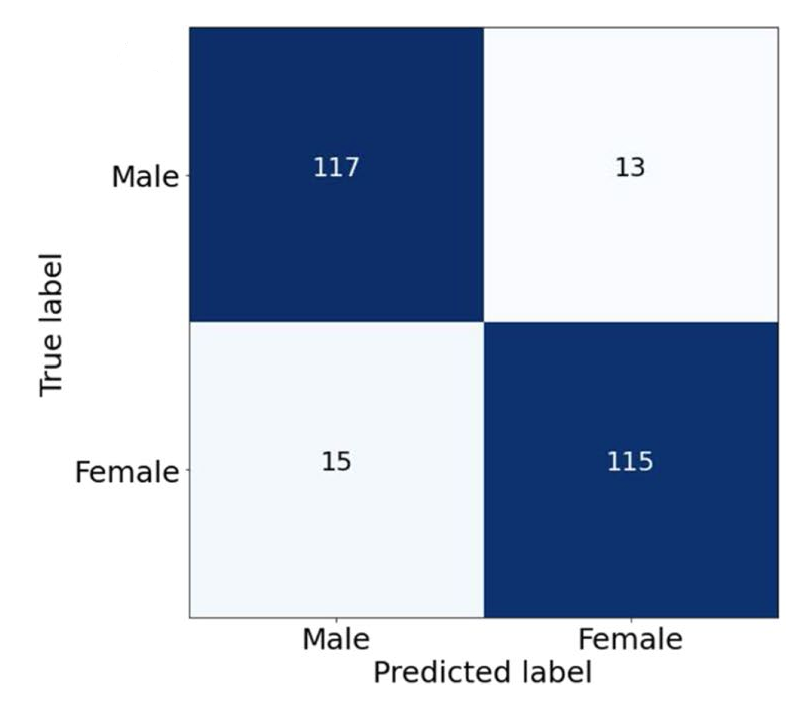
\includegraphics[width=0.6\textwidth]{capitulos/cap_02/imagenes/confusion_matrix_binary.png}
        \caption{
            Matriz de confusión para la estimación de sexo según el modelo \textit{random forest} propuesto en \cite{bidmos2023}.
        } 
        \label{fig:conf_matrix_binary}
    \end{figure}

    \item La \textbf{exactitud (\textit{accuracy})} es la proporción de instancias totales bien clasificadas. 
    
    % \begin{figure}[h]
    %     \centering
    
    %     \begin{subfigure}[b]{0.3\textwidth}
    %         \centering
    %         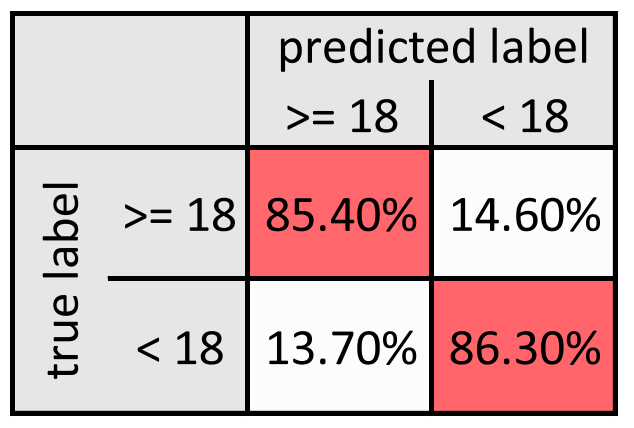
\includegraphics[width=\textwidth]{capitulos/cap_02/imagenes/confusion_matrix_binary_1.png}
    %         \caption{Sin información de sexo}
    %         \label{fig:conf_matrix_general}
    %     \end{subfigure}
    %     \hfill
    %     \begin{subfigure}[b]{0.3\textwidth}
    %         \centering
    %         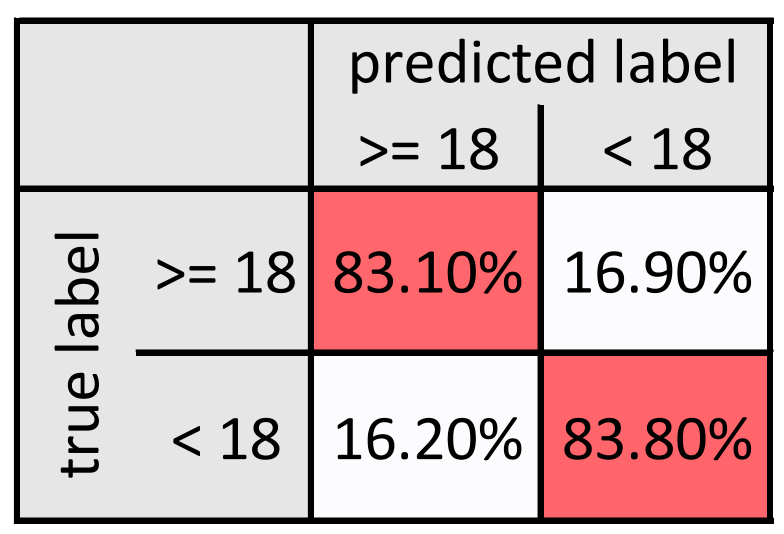
\includegraphics[width=\textwidth]{capitulos/cap_02/imagenes/confusion_matrix_binary_2.png}
    %         \caption{Sexo femenino}
    %         \label{fig:conf_matrix_female}
    %     \end{subfigure}
    %     \hfill
    %     \begin{subfigure}[b]{0.3\textwidth}
    %         \centering
    %         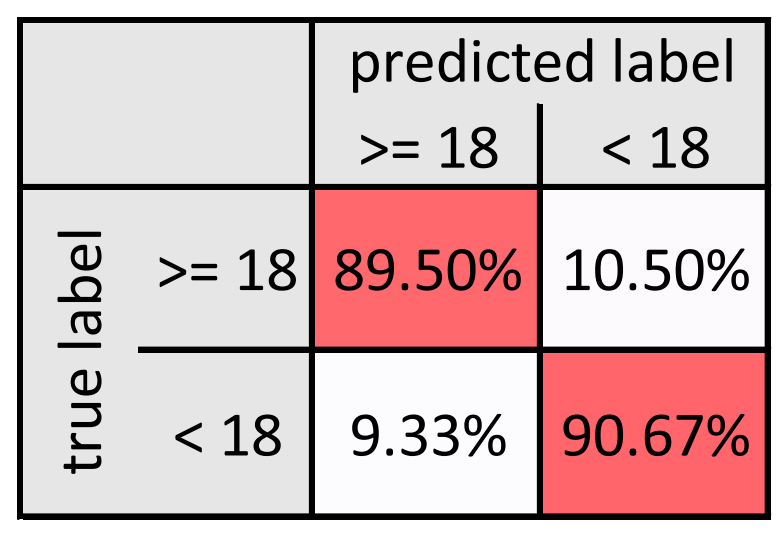
\includegraphics[width=\textwidth]{capitulos/cap_02/imagenes/confusion_matrix_binary_3.png}
    %         \caption{Sexo masculino}
    %         \label{fig:conf_matrix_male}
    %     \end{subfigure}
    
    %     \caption[
    %         Matrices de confusión para la estimación de mayoría/minoría de edad según el modelo de 
    %         \cite{porto2020}.
    %     ]{
    %         Matrices de confusión para la estimación de mayoría/minoría de edad según el modelo de 
    %         \cite{porto2020}.
    %         Se representan los valores de cada celda en términos porcentuales de los ejemplos reales que hay 
    %         de cada clase ($< 18$ y $\ge 18$), lo que permite comparar la matriz de confusión general de todos 
    %         los ejemplos (\ref{sub@fig:conf_matrix_general}) con la de ejemplos se sexo femenino 
    %         (\ref{sub@fig:conf_matrix_female}) y sexo masculino (\ref{sub@fig:conf_matrix_male}), permitiendo 
    %         identificar posibles sesgos en el modelo respecto al género, y así realizar una evaluación más 
    %         precisa del rendimiento del modelo en diferentes subgrupos de la población.
    %     }
    %     \label{fig:conf_matrix_binary_relative}

    % \end{figure}

\end{itemize}


Por otro lado, para la clasificación multietiqueta emplearemos:

\begin{itemize}

    \item La \textbf{cobertura empírica (\textit{empirical coverage})}, de forma análoga a la regresión, mide la proporción de veces que la etiqueta verdadera está contenida dentro del conjunto predicho.

    $$
    EC = \frac{1}{n} \sum_{i=1}^{n} \mathbb{I}(y_i \in \Gamma_\alpha(x_i))
    $$

    Esta variable se puede obtener o bien en todos los ejemplos del conjunto, o en subpoblaciones específicas de este.

    \item Se denomina \textbf{violación de la cobertura empírica (\textit{empirical coverage violation})} a la magnitud en que la cobertura empírica no alcanza el nivel de cobertura teórico deseado $1 - \alpha$, definida como:

    $$
    ECV = max \left\{ 0,(1-\alpha)-EC \right\}
    $$

    Este valor cuantifica cuánto se desvía el método de la garantía nominal
    \footnote{
        Se denomina garantía de cobertura nominal al nivel de cobertura garantizado estadísticamente.
    } 
    cuando no se alcanza la cobertura esperada. Una violación igual a cero indica que el método cumple o supera el nivel de cobertura deseado.

    Esta métrica se suele calcular sobre subconjuntos específicos del conjunto de instancias para evaluar la cobertura condicional, es decir, la calidad de la cobertura dentro de subpoblaciones del dominio.

    \item El \textbf{tamaño medio de conjunto de predicción (\textit{mean prediction set size})} mide cuántas etiquetas, en promedio, incluyen los conjuntos de predicción conformales $\Gamma_\alpha(x)$.

    $$
    MSS = \frac{1}{n} \sum_{i=1}^n | \Gamma_\alpha(x_i) |
    $$

    % \item Gráfico de barras de violación de cobertura en base al tamaño del conjunto (inspirada en la métrica \textit{Each-Size Coverage Violation} propuesta en \cite{huang2023conformal}): En esta gráfica, para cada tamaño posible del conjunto de predicción, se calcula la violación de cobertura empírica correspondiente, es decir, cuánto se desvía la cobertura observada respecto al nivel nominal $(1 - \alpha)$. Esto permite visualizar en qué tamaños de conjunto el modelo tiende a fallar más en cuanto a cobertura, proporcionando una forma más detallada de analizar el comportamiento del método conforme más allá de la cobertura global.

    
\end{itemize}


Y, finalmente, también usaremos elementos visuales para valorar el desempeño de las predicciones interválicas:

\begin{itemize}

    \item \textbf{Gráfica de dispersión de Cobertura Empírica - Tamaño Medio del Conjunto de Predicción}: Este gráfico permite visualizar el compromiso entre cobertura lograda y tamaño del intervalo. Un buen modelo debería situarse cerca del nivel de confianza objetivo con intervalos lo más cortos posible. 

    \item \textbf{Histograma de tamaños de conjuntos de predicción}: 

    \item  \textbf{Gráfica de barras de cobertura en base al tamaño del conjunto}. Esta gráfica muestra la cobertura empírica lograda para cada tamaño del conjunto de predicción. Esto permite visualizar en qué tamaños de conjunto el modelo tiende a infracubir o sobrecubrir más en cuanto a cobertura.

\end{itemize}
